\section{Mitarbeieransicht}

\subsection{Vorhandene Technologien}
Für das Projekt stehen die folgenden populären Webframeworks zur Verfügung: \textbf{Angular}, \textbf{React}, \textbf{Vue.js} und \textbf{Next.js}. Diese bilden die Grundpfeiler der Webentwicklung weltweit und werden von unzähligen Organisationen aktiv verwendet und empfohlen.

\begin{figure}
	\centering
	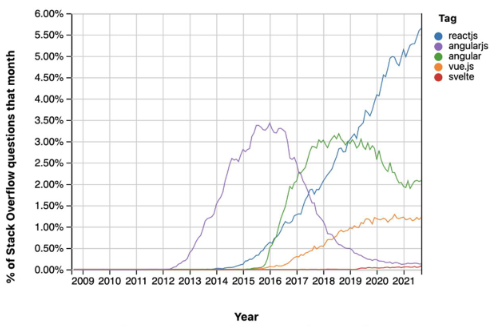
\includegraphics[width=0.85\textwidth]{images/framework_popularity.png}
	\caption{zeigt die Popularität verschiedener Frontend-Frameworks über die Jahre, basierend auf dem Anteil der Fragen auf Stack Overflow. \textit{\cite{akivab_js_framework}}}
\end{figure}


\subsubsection{Angular}

\textbf{Einführung in Angular}
\newline
Angular ist ein quelloffenes Framework für die Frontend-Webentwicklung, das von Google entwickelt wurde. Es wurde erstmals 2010 als AngularJS eingeführt und mit Angular 2 vollständig überarbeitet. Es basiert auf TypeScript und ermöglicht die Erstellung dynamischer, skalierbarer Single-Page-Anwendungen (SPAs). Durch regelmäßige Updates bleibt Angular ein modernes Framework, das an die Anforderungen der Webentwicklung angepasst ist.\textit{\cite{madurapperuma2022state, shetty2020review, angular}} \newline


\textbf{Architektur}
\newline
Angular verwendet eine komponentenbasierte Architektur, bei der die Benutzeroberfläche in kleine, wiederverwendbare Teile (Komponenten) unterteilt wird. Jede Komponente besteht aus:

\begin{itemize}
	\item \textbf{Templates}: HTML, erweitert mit Angular-spezifischen Direktiven.
	\item \textbf{Styles}: CSS oder SCSS für das Design.
	\item \textbf{Logik}: TypeScript für die Geschäftslogik.
\end{itemize}

Komponenten werden in Modulen (\text{NgModules}) gruppiert, um eine bessere Organisation und Wiederverwendbarkeit zu gewährleisten. Diese Struktur fördert die Modularität und erleichtert die Wartung des Codes.\textit{\cite{hutagikar2020analysis, shetty2020review, angular}} \newline

\textbf{Hauptfunktionen von Angular}

\textbf{Datenbindung} 

Angular unterstützt sowohl Einweg- als auch Zweiweg-Datenbindung:

\begin{itemize}
	\item \textbf{Einweg-Datenbindung}: Daten fließen nur vom Model zur View.
	\item \textbf{Zweiweg-Datenbindung}: Änderungen in der View werden automatisch an das Model zurückgegeben und umgekehrt. Dies wird häufig für Formulare verwendet und reduziert den manuellen Aufwand bei der Synchronisation.\textit{\cite{hutagikar2020analysis, madurapperuma2022state, angular}}
\end{itemize}

\textbf{Vorteile von Angular}
\begin{itemize}
	\item \textbf{Skalierbarkeit}: Angular eignet sich sowohl für kleine als auch für große Projekte, dank seiner Modularität und TypeScript-Unterstützung.\textit{\cite{madurapperuma2022state, rathinam2022analysis, angular}}
	
	\item \textbf{Integrierte Tools}: Angular CLI (Command Line Interface) erleichtert die Projektinitialisierung, den Build-Prozess und das Testen. Angular Material bietet vorgefertigte UI-Komponenten, die das Design beschleunigen.\textit{\cite{hutagikar2020analysis, angular_blog}}
	
	\item \textbf{Community und Support}: Als von Google unterstütztes Framework verfügt Angular über eine aktive Entwicklergemeinschaft, regelmäßige Updates und umfassende Dokumentation.\textit{\cite{shetty2020review, angular}}
\end{itemize}

\textbf{Nachteile von Angular}
\begin{itemize}
	\item \textbf{Steile Lernkurve}: Durch die Einführung von TypeScript, Dependency Injection und einer komplexen Struktur ist Angular für Anfänger herausfordernd.\textit{\cite{madurapperuma2022state, rathinam2022analysis, angular_blog}}
	\item \textbf{Framework-Größe}: Angular ist im Vergleich zu leichtgewichtigen Frameworks wie Vue.js oft schwerer und kann dadurch die Ladezeit beeinflussen.\textit{\cite{shetty2020review, angular}}
\end{itemize}


\subsubsection{React}

\textbf{Einführung in React}
\newline
React ist eine quelloffene JavaScript-Bibliothek, die von Meta (ehemals Facebook) entwickelt wurde und hauptsächlich zur Erstellung von Benutzeroberflächen verwendet wird. Sie wurde erstmals 2013 veröffentlicht und ist besonders für die Entwicklung dynamischer Single-Page-Anwendungen (SPAs) geeignet. React basiert auf dem Konzept von Komponenten und der Verwendung eines virtuellen DOM, um die Performance zu optimieren. Es bietet eine flexible Architektur für die Entwicklung moderner Webanwendungen.\textit{\cite{rathinam2022analysis, hutagikar2020analysis, react}} \newline

\textbf{Architektur}
\newline
React verwendet eine komponentenbasierte Architektur, bei der Benutzeroberflächen in kleinere, wiederverwendbare Teile aufgeteilt werden. Diese Architektur ermöglicht eine einfache Wartung und Erweiterung von Anwendungen. Jede Komponente in React ist in JSX (JavaScript XML) geschrieben, einer Syntaxerweiterung, die HTML-ähnlichen Code innerhalb von JavaScript erlaubt.

\begin{itemize}
	\item \textbf{Virtueller DOM}: React verwendet einen virtuellen DOM, der Änderungen an der Benutzeroberfläche effizient berechnet und nur die betroffenen Teile des echten DOM aktualisiert.
	\item \textbf{JSX}: JSX ist eine Mischung aus JavaScript und HTML, die es Entwicklern ermöglicht, benutzerdefinierte UI-Komponenten zu erstellen.
	\item \textbf{Unidirektionaler Datenfluss}: Daten fließen in React in einer einzigen Richtung, was die Verwaltung und Nachverfolgbarkeit von Daten einfacher macht.\textit{\cite{rathinam2022analysis, hutagikar2020analysis, react}}
\end{itemize}

\textbf{Hauptfunktionen von React}

\textbf{Komponentenbasierte Entwicklung} 

React ermöglicht die Erstellung von wiederverwendbaren und modularen Komponenten, die sowohl die Benutzeroberfläche als auch die Logik kapseln. Dies fördert eine bessere Strukturierung und Wartbarkeit des Codes.\textit{\cite{shetty2020review, react}}

\textbf{Virtueller DOM} 

Der virtuelle DOM verbessert die Performance von React-Anwendungen, indem er Änderungen effizient berechnet und nur die betroffenen Teile des echten DOM aktualisiert. Dies reduziert die Anzahl der direkten DOM-Manipulationen erheblich.\textit{\cite{rathinam2022analysis, hutagikar2020analysis, react}}

\textbf{Vorteile von React}
\begin{itemize}
	\item \textbf{Performance}: Der virtuelle DOM und die asynchrone Verarbeitung ermöglichen eine schnelle und effiziente Benutzeroberfläche.\textit{\cite{rathinam2022analysis, react}}
	
	\item \textbf{Flexibilität und Wiederverwendbarkeit}: Die komponentenbasierte Architektur von React erleichtert die Wiederverwendung von Code und die Skalierung von Anwendungen.\textit{\cite{hutagikar2020analysis, react}}
	
	\item \textbf{Große Community und Ökosystem}: React wird von einer riesigen Entwicklergemeinschaft unterstützt, und es gibt zahlreiche Bibliotheken und Tools, die den Entwicklungsprozess verbessern.\textit{\cite{shetty2020review, react}}
\end{itemize}

\textbf{Nachteile von React}
\begin{itemize}
	\item \textbf{Zusätzliche Abhängigkeiten}: React bietet nur die grundlegende Architektur, weshalb oft zusätzliche Bibliotheken (z. B. für Routing oder State Management) benötigt werden.\textit{\cite{shetty2020review, rathinam2022analysis, react_blog}}
	
	\item \textbf{Lernkurve}: Für Entwickler, die mit JSX und der Unidirektionalität des Datenflusses nicht vertraut sind, kann React eine gewisse Lernkurve darstellen.\textit{\cite{hutagikar2020analysis, react_blog}}
\end{itemize}



\subsubsection{Vue.js}

\textbf{Einführung in Vue.js}
\newline
Vue.js ist ein progressives JavaScript-Framework, das 2014 von Evan You entwickelt wurde. Es wird häufig für die Erstellung von Benutzeroberflächen und Single-Page-Anwendungen (SPAs) verwendet. Vue.js zeichnet sich durch seine einfache Integration in bestehende Projekte und seine Flexibilität aus, wodurch es sowohl für kleine als auch große Anwendungen geeignet ist. Durch seine modulare Struktur und starke Community-Unterstützung bleibt Vue.js ein beliebtes Framework für Webentwickler.\textit{\cite{rathinam2022analysis, madurapperuma2022state, vuejs}} \newline

\textbf{Architektur}
\newline
Vue.js verwendet die Model-View-ViewModel (MVVM)-Architektur, die es ermöglicht, die Benutzeroberfläche, die Geschäftslogik und die Datenbindung effizient zu verwalten. Die Hauptbestandteile von Vue.js sind:

\begin{itemize}
	\item \textbf{Templates}: Vue.js verwendet Templates, um UI-Komponenten zu definieren. Diese Templates werden in renderbare DOM-Elemente übersetzt.
	\item \textbf{Reaktivitätssystem}: Das reaktive Datenmodell von Vue.js ermöglicht automatische Updates der Benutzeroberfläche, wenn sich die zugrunde liegenden Daten ändern.
	\item \textbf{Direktiven}: Vue.js bietet spezielle HTML-Attribute (Direktiven), die Funktionen wie Schleifen, Bedingungen und Ereignishandlungen erleichtern.\textit{\cite{hutagikar2020analysis, vuejs}}
\end{itemize}

\textbf{Hauptfunktionen von Vue.js}

\textbf{Komponentenbasierte Entwicklung} 

Wie React und Angular ermöglicht Vue.js die Erstellung von wiederverwendbaren und modularen Komponenten. Diese Struktur fördert die Organisation und erleichtert die Wartung und Erweiterung von Anwendungen.\textit{\cite{rathinam2022analysis, vuejs}}

\textbf{Reaktivitätssystem} 

Das Reaktivitätssystem von Vue.js überwacht automatisch Änderungen im Datenmodell und aktualisiert die Benutzeroberfläche entsprechend. Dies macht die manuelle DOM-Manipulation überflüssig und verbessert die Entwicklererfahrung.\textit{\cite{hutagikar2020analysis, vue_blog}}

\textbf{Vorteile von Vue.js}
\begin{itemize}
	\item \textbf{Einfache Lernkurve}: Vue.js ist einfach zu lernen, da es eine klare und intuitive Syntax bietet. Es ist besonders für Entwickler geeignet, die mit HTML, CSS und JavaScript vertraut sind.\textit{\cite{madurapperuma2022state, vuejs}}
	
	\item \textbf{Flexibilität und Modularität}: Vue.js kann sowohl für einfache Widgets als auch für komplexe Anwendungen verwendet werden. Seine modulare Struktur ermöglicht eine einfache Integration in bestehende Projekte.\textit{\cite{rathinam2022analysis, vuejs}}
	
	\item \textbf{Leichtgewichtig und performant}: Vue.js ist kleiner als Frameworks wie Angular und React, was die Ladezeit reduziert und die Performance verbessert.\textit{\cite{shetty2020review, vuejs}}
\end{itemize}

\textbf{Nachteile von Vue.js}
\begin{itemize}
	\item \textbf{Geringere Unterstützung durch große Unternehmen}: Im Gegensatz zu React und Angular wird Vue.js nicht von einer großen Organisation unterstützt, was in einigen Fällen zu Unsicherheiten führen kann.\textit{\cite{rathinam2022analysis, vue_blog}}
	
	\item \textbf{Weniger umfangreiches Ökosystem}: Während Vue.js eine starke Community hat, sind bestimmte Drittanbieter-Bibliotheken und Tools im Vergleich zu React und Angular weniger verbreitet.\textit{\cite{hutagikar2020analysis, vue_blog}}
\end{itemize}


\subsubsection{Next.js}

\textbf{Einführung in Next.js}
\newline Next.js ist ein populäres Open-Source-React-Framework, das 2016 von Vercel entwickelt wurde. Es erleichtert die Erstellung von Server-Rendered-Anwendungen und bietet Funktionen wie statische Seitengenerierung, serverseitiges Rendering und dynamisches Routing. Mit seiner Optimierung für Entwicklererfahrung und seiner Flexibilität ist Next.js eine bevorzugte Wahl für moderne Webprojekte und eignet sich sowohl für einfache als auch komplexe Anwendungen. Dank seiner Performance-Vorteile und Integration mit React bleibt es eine wichtige Technologie im Bereich der Webentwicklung.\textit{\cite{nextjs, rathinam2022analysis, shetty2020review}}

\textbf{Architektur}
\newline Next.js verwendet eine komponentenbasierte Architektur, die auf React aufbaut und eine erweiterte Struktur zur effizienten Verwaltung von Benutzeroberflächen und Backend-Interaktionen bereitstellt. Die Hauptbestandteile von Next.js sind:
\begin{itemize} \item \textbf{Pages und Routing}: Jede Datei in der \texttt{pages}-Ordnerstruktur entspricht einer Route. Next.js unterstützt sowohl statische als auch dynamische Routen. \item \textbf{Serverseitiges Rendering (SSR)}: Ermöglicht die Generierung von Inhalten auf dem Server, bevor sie an den Client gesendet werden. \item \textbf{Statische Seitengenerierung (SSG)}: Statische Seiten werden zur Build-Zeit generiert, was die Performance und SEO optimiert.\textit{\cite{nextjs, nextjs_blog, rathinam2022analysis}} \end{itemize}

\textbf{Hauptfunktionen von Next.js}

\textbf{Server-Rendering und Statische Generierung}
Next.js kombiniert serverseitiges Rendering und statische Seitengenerierung, um Entwicklern die Flexibilität zu bieten, die beste Strategie für ihre Anwendung zu wählen. Diese Funktionen fördern die Performance und SEO.\textit{\cite{nextjs, nextjs_blog, shetty2020review}}

\textbf{Integrierte Optimierungen}
Next.js bietet Funktionen wie automatisches Code-Splitting, \newline
Image-Optimierung und automatische Routing-Updates, die eine effiziente und moderne Entwicklungserfahrung fördern.\textit{\cite{nextjs, rathinam2022analysis, nextjs_blog}}

\textbf{Vorteile von Next.js}
\begin{itemize} \item \textbf{SEO-Optimierung}: Server-Rendering und statische Generierung tragen zur Verbesserung der Suchmaschinenplatzierung bei.\textit{\cite{nextjs, nextjs_blog, shetty2020review}} \item \textbf{Hohe Performance}: Durch Funktionen wie automatische Code-Splitting und Bildoptimierung bietet Next.js schnelle Ladezeiten und eine optimale Benutzererfahrung.\textit{\cite{rathinam2022analysis, nextjs, shetty2020review}} \item \textbf{Flexibilität}: Die Unterstützung für verschiedene Rendering-Strategien und die Integration mit React ermöglichen den Einsatz für eine Vielzahl von Anwendungsfällen.\textit{\cite{nextjs_blog, nextjs, shetty2020review}} \end{itemize}

\textbf{Nachteile von Next.js}
\begin{itemize} \item \textbf{Steile Lernkurve}: Insbesondere für Entwickler ohne Erfahrung mit React kann die Einarbeitung in Next.js herausfordernd sein.\textit{\cite{rathinam2022analysis, shetty2020review}} \item \textbf{Build-Zeiten}: Bei sehr großen Projekten können die Build-Zeiten länger dauern, was die Entwicklungszyklen beeinflusst.\textit{\cite{madurapperuma2022state, rathinam2022analysis}} \end{itemize}


